\documentclass{article} % For LaTeX2e
\usepackage{nips12submit_e,times}
\usepackage{graphicx}
\usepackage{amsmath}
\usepackage{amssymb}
\usepackage{multirow}
%\documentstyle[nips12submit_09,times,art10]{article} % For LaTeX 2.09

\usepackage{graphicx}
\graphicspath{{./figures/}}
\title{Homework based on Chapter 17, 19\\
Computational Probability and Statistics \\
CIS 2033, Section 002}
\author{Due: 9:00 AM, Friday, April 17, 2015}


% The \author macro works with any number of authors. There are two commands
% used to separate the names and addresses of multiple authors: \And and \AND.
%
% Using \And between authors leaves it to \LaTeX{} to determine where to break
% the lines. Using \AND forces a linebreak at that point. So, if \LaTeX{}
% puts 3 of 4 authors names on the first line, and the last on the second
% line, try using \AND instead of \And before the third author name.

\newcommand{\fix}{\marginpar{FIX}}
\newcommand{\new}{\marginpar{NEW}}

\nipsfinalcopy % Uncomment for camera-ready version

\begin{document}

\maketitle

\paragraph*{17.4} 
\begin{figure}[h!]
\centering
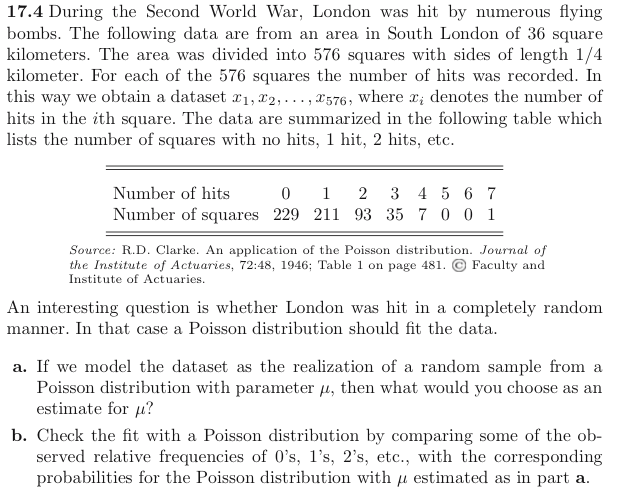
\includegraphics[width=5.5in, height=4.5in]{1.png}
\end{figure}

\subparagraph*{a.} Let the random variable $X$ denote the number of hits and $X \sim Pois(\mu)$. Then $E[X] = \mu$. 
\begin{align*}
\mu & = \frac{0\times 229 + 1\times 211 + 2\times 93 + 3 \times 35 + 4 \times 7 + 5 \times 0 + 6\times 0 + 7\times 1}{576}\\
& = \frac{537}{576} = 0.9323
\end{align*}

\subparagraph*{b.} 
We compute the frequency by using $\text{freq}(k)=\frac{\#squares in k hits}{\#total squares:576}$ and compute the probability by using $P(X=k) = \frac{\mu^k}{k!}e^{-\mu}$, for $k=0,1, \ldots, 7$ where $\mu =0.9323$, 
\begin{table}[h!]
\centering
\begin{tabular}{ccccccccc} \\ \hline \hline 
\# hits & 0 & 1 & 2 & 3 & 4 & 5 & 6 & 7 \\ \hline
\# squares & 229 & 211 & 93 & 35 & 7 & 0 & 0 & 1 \\ \hline
$\text{freq}=\frac{\#squares}{\#total squares:576}$ &
0.3976 & 0.3663  &   0.1615   &  0.0608  &   0.0122    &     0    &     0  &  0.0017\\
$P(X=k) = \frac{\mu^k}{k!}e^{-\mu}$ & 
 0.3936  &  0.3670  &  0.1711  &  0.0532 &   0.0124  &  0.0023  &  0.0004 &   0.0000 \\
\hline \hline
\end{tabular}
\end{table}

\paragraph*{17.6} 
\begin{figure}[h!]
\centering
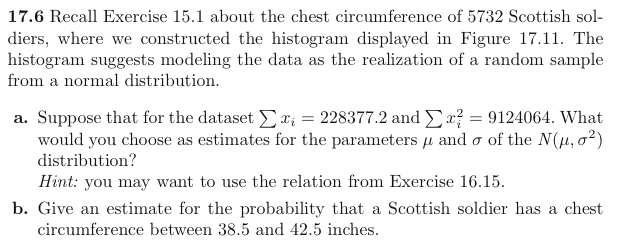
\includegraphics[width=5.5in, height=3in]{2.png}\\
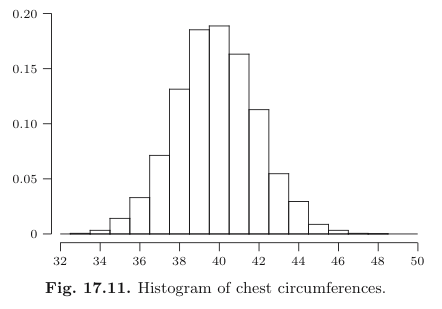
\includegraphics[width=3in, height=2in]{3.png}\\
\end{figure}

\subparagraph*{a.}
$N(\mu, \sigma^2)$, we can 
\begin{align*}
\mu  & = \frac{1}{n}\sum_i x_i = \frac{1}{5732} 228377.2 =  39.8425 \\
\sigma & = \sqrt{\frac{1}{n-1} \sum_i \left( x_i - \mu \right)^2}  \\
& = \sqrt{\frac{1}{n-1} \sum_i \left( x_i ^2 + \mu^2 - 2\mu x_i\right)} \\
& = \sqrt{\frac{1}{n-1} \sum_i x_i^2 + \sum_i \mu^2 - \sum_i 2\mu x_i}\\
& = \sqrt{\frac{1}{n-1} \sum_i x_i^2 +  n \mu^2 - 2\mu \sum_i x_i}\\
& = \sqrt{\frac{1}{5732-1} 9124064 + 5732(39.8425)^2 - 2(39.8425) 228377.2 }\\
& =   2.0863
\end{align*}

\subparagraph*{b.}
Given $X \sim N(\mu, sigma^2)$, where $\mu=39.8425, \sigma^2=4.3526$, let $Z = \frac{X-\mu}{\sigma}$, and $Z$ is a standard norm distribution such that $Z \sim N(0, 1)$. We have to compute 
\begin{align*}
P(38.5<X<42.5) & = P(X<42.5) - P(X < 38.5) \\
& = P(Z < \frac{42.5-\mu}{\sigma}) - P(Z < \frac{38.5-\mu}{\sigma})\\
& = \Phi(\frac{42.5-\mu}{\sigma}) - \Phi(\frac{38.5-\mu}{\sigma}) \\
& = \Phi(1.2738) - \Phi( -0.6435) \\
& = 0.8980 - 0.2611 \\
& = 0.6369
\end{align*}
Note that $\Phi(1.2738)=P(Z\leq 1.2738) = 1-\hat{p}$, where $\hat{p}$ is the value obtained from the lookup table; 
$\Phi(-0.6435) = P(Z \leq -0.6435) = P(Z \geq 0.6435) = \tilde{p}$ where $\tilde{p}$ is the valued obtained from the lookup table. 

\paragraph*{19.2} Suppose the random variables $X_1, X_2, \ldots, X_n$ have the same expectation $\mu$. 
\subparagraph*{a.} Is $S=\frac{1}{2}X_1 + \frac{1}{3}X_2 + \frac{1}{6}X_3$ an unbiased estimator for $\mu$ ?
\subparagraph*{b.} Under what conditions on constants $a_1, a_2, \ldots, a_n$ is $T=a_1X_1 + a_2 X_2 + \ldots a_nX_n$ an unbiased estimator for $\mu$ ?

{\bf For a)}, $E[S] = E[\frac{1}{2}X_1 + \frac{1}{3}X_2 + \frac{1}{6}X_3] = \frac{1}{2}E[X_1] + \frac{1}{3}E[X_2] +\frac{1}{6}E[X_3] = \frac{1}{2}\mu + \frac{1}{3}\mu + \frac{1}{6}\mu = \mu$. So, $S$ is unbiased estimator for $\mu$. 

{\bf For b)}, $T$ is an unbiased estimator for $\mu$, then $E[T] = \mu$. Then, $E[T]=E[a_1X_1 + a_2 X_2 + \ldots a_nX_n] = a_1E[X_1] + a_2 E[X_2] + \ldots + a_nE[X_n] = a_1\mu + a_2 \mu + ldots + a_n \mu + \left( a_1 + a_2 + \ldots + a_n\right) \mu = \mu $, then $a_1 + a_2 + \ldots + a_n = 1$. 

\paragraph*{19.5} Suppose a dataset is modeled as a realization of a random sample $X_1, X_2, \ldots, X_n$ from an $Exp(\lambda)$ distribution, where $\lambda >0 $ is unknown. Let $\mu$ denote the corresponding expectation and let $M_n$ denote the minimum of $X_1, X_2, \ldots, X_n$. Recall that $M_n$ has an $Exp(n\lambda)$ distribution. Find out for which constant $c$ the estimator $T=cM_n$ is an unbiased estimator for $\mu$. 

We know that $E[M_n] = \frac{1}{n\lambda}$ since $M_n \sim Exp(n\lambda)$. \\
Then $E[T] = E[cM_n] = cE[M_n] = \frac{c}{n\lambda}$. Let $T$ be an unbiased estimator for $\mu$, then $E[T] = \mu$, then $\frac{c}{n\lambda}=\mu$, then $c= n \lambda \mu$. Moreover, from the question, we know that $\mu$ is the expectation of a $Exp(\lambda)$, then $\mu = \frac{1}{\lambda}$. Then, $c = n$. 

\paragraph*{19.7}
\begin{figure}[h!]
\centering
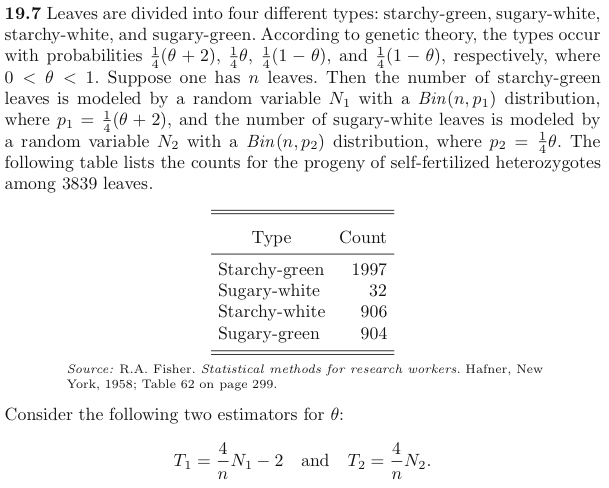
\includegraphics[width=5.5in, height=4.5in]{4.png}
\end{figure}
\subparagraph*{a.} Check that both $T_1$ and $T_2$ are unbiased estimator for $\theta$. 
\subparagraph*{b.} Compute the value of both estimators for $\theta$. 

{\bf For a)}, $E[T_1] = E[\frac{4}{n}N_1 - 2] = \frac{4}{n}E[N_1] - 2 = \frac{4}{n} np_1 - 2 = \frac{4}{n}n\frac{1}{4}(\theta + 2) - 2 = \theta + 2 - 2 = \theta$. So, $T_1$ is an unbiased estimator for $\theta$. 

$E[T_2] = E[\frac{4}{n}N_2]=\frac{4}{n}E[N_2] = \frac{4}{n}np_2 = \frac{4}{n}n\frac{1}{4}\theta = \theta$. So, $T_2$ is an unbiased estimator for $\theta$. 

{\bf b)}, $n = 3839, n_1 = 1997, n_2 = 32, E[N_1] = 1997, E[N_2] = 32$,
$E[T_1] = \frac{4}{n}E[N_1] - 2 = \frac{4}{3839}1997  - 2 = 0.0808$. \\
$E[T_2] = \frac{4}{n}E[N_2] = \frac{4}{3839}32 = 0.0333$.

\end{document}
